\documentclass{article}

\usepackage[margin=1in]{geometry}
\usepackage{lipsum}
\usepackage{graphicx}
\usepackage{amsmath}

\begin{document}
    \title{Mastering Algorithms with C}
    \maketitle

    \tableofcontents

    \section{Hash Tables}
    
    The primary idea behind a hash table is to establish a mapping between the set of all possible keys and positions in the array using a hash function, which returns the hash coding/hash value of the key.

    \subsection{chained hash tables}

    A chained hash table fundamentally consists of an array of linked lists. Each list forms a bucket in which we place all elements hashing to a specific position in the array. To insert an element, we first pass its key to a hash function in a process called hashing the key, then we insert the element at the head of the appropriate list. To look up or remove an element, we hash its key again to find its bucket, then traverse the appropriate list until we find the element we are looking for.
    \begin{figure}[h]
    \centering
    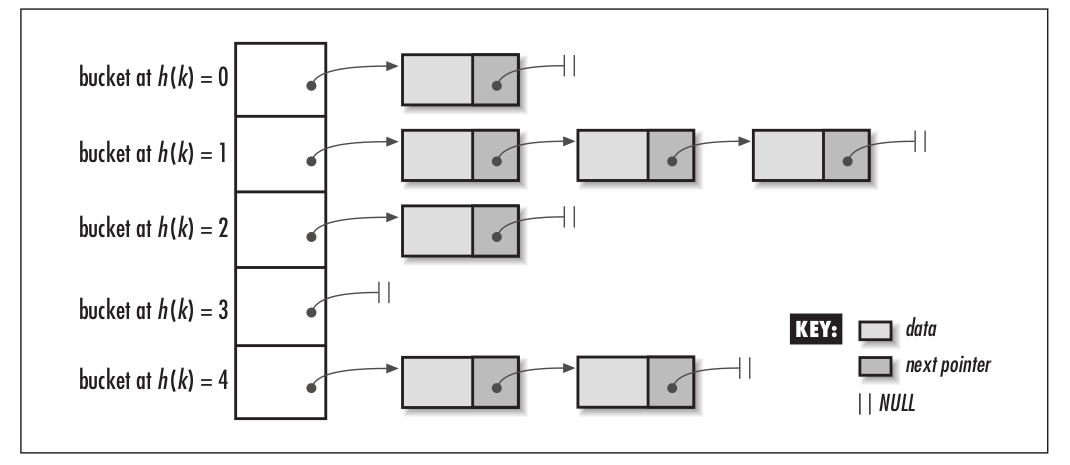
\includegraphics[width=0.5\linewidth]{images/hash-tables-1}
    \caption{A chained hash table with five buckets containing a total of seven elements}
    \end{figure}

    When two keys hash to the same position in a hash table, they collide. Chained hash tables have a simple solution for resolving collisions: elements are simply placed in the bucket where the collision occurs. One problem with this, however, is that if an excessive number of collisions occur at a specific position, a bucket becomes longer and longer, taking more time to access the elements.
    \subsection{open addressed hash tables}

    In an chained hash table, elements reside in buckets extending from each position. In an open-addressed hash table, on the other hand, all elements reside in the table itself. This may be important for some applications that rely on the table being a fixed size.

    The way to resolve collisions in an open addressed hash table is to probe the table. To insert an element, for example, we probe positions until we find an unoccupied one, and insert the element there. To remove or look up an element, we probe positions until the element is located or until we encounter an unoccupied position. If we encounter an unoccupied position before finding the element, or if we end up traversing all of the positions, the element is not in the table.

    Generally, a hash function for probing positions in an open addressed hash table is defined by:
    $$
    h(k,i) = x
    $$
    where $k$ is a key, $i$ is the number of times the table has been probed thus far, and $x$ is the resulting hash coding. For an open addressed hash table, $h$ must possess an additional property: as $i$ increases from 0 to $m - 1$, where $m$ is the number of positions in the hash table, all positions in the table must be visited before any position is visited twice, otherwise, not all positions will be probed.

    \subsubsection{linear probing}
    
    One simple approach to probing an open addressed hash table is to probe successive positinos in the table. If we let $i$ go between 0 and $m - 1$, where $m$ is the number of positions in the table, a hash function for linear probing is defined as:
    $$
    h(k,i) = (h'(k) + i) \mod m
    $$
    The function $h'$ is an auxiliary hash function, which is selected like any hash function. For example, we might choose to use the division method of hashing and let $h'(k) = k \mod m$, in this case, if we hash an element with key $k = 2998$ into a table of size $m = 1000$, the hash codings produced are (998 + 0) mod 1000 = 0 when $i = 0$, (998 + 1) mod 1000 = 999 when $i = 1$, (998 + 2) mod 1000 = 0 when $i = 2$, and so on. The advantage of linear probing is that it is simple and there are no constraints on $m$ to ensure that all positions will eventually be probed. Unfortunately, linear probing does not approximate uniform hashing very well, in particular, linear probing suffers from a phenomenon known as primary clustering, in which large chains of occupied positions begin to develop as the table becomes more and more full, this results in excessive probing.
    \begin{figure}[h]
    \centering
    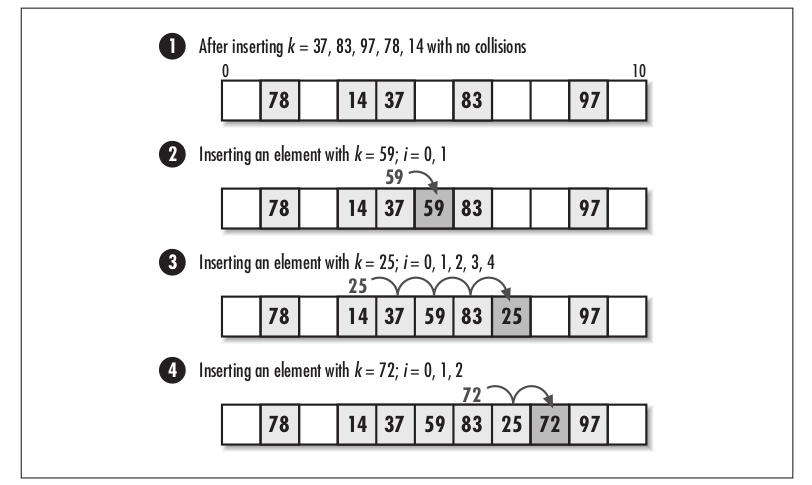
\includegraphics[width=0.5\linewidth]{images/hash-tables-2}
    \caption{linear probing with $h(k,i) = (k \mod 11 + i) \mod 11$}
    \end{figure}

    \subsubsection{double hashing}

    One of the most effective approaches for probing an open-addressed hash table focuses on adding the hash codings of two auxiliary hash functions. If we let $i$ go between 0 and $m - 1$, where $m$ is the number of positions in the table, a hash function for double hashing is defined as:
    $$
    h(k,i) = (h_1(k) + ih_2(k)) \mod m
    $$
    The functions $h_1$ and $h_2$ are auxiliary hash functions, which are selected like any hash function. In order to ensure that all positions in the table are visited before any position is visited twice, we must adhere to one of the following procedures: we must select $m$ to be a power of 2 and make $h_2$ always return an odd value, or we must make $m$ prime and design $h_2$ so that it always return a positive integer less than $m$.

    Typically, we let $h_1(k) = k \mod m$ and $h_2(k) = 1 + (k \mod m')$, where $m'$ is slightly less than $m$, say, $m - 1$ or $m - 2$. Using this approach, for example, if the hash table contains $m = 1699$ positions (a prime number) and we hash the key $k = 15385$, the positions probed are $(94 + (0)(113)) \mod 1699 = 94$ when $i = 0$, and every 113th position after this as $i$ increases.
    \begin{figure}[h]
    \centering
    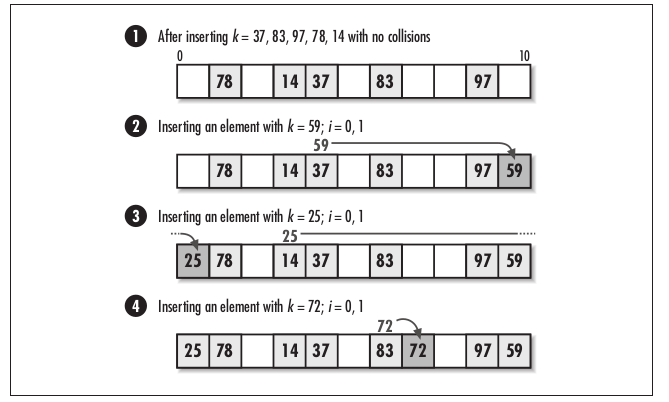
\includegraphics[width=0.5\linewidth]{images/hash-tables-3}
    \caption{hashing with double hashing}
    \end{figure}

\end{document}
